\section{Kiến thức nền tảng}
\subsection{Các công nghệ về Frontend}
\subsubsection{HTML (HyperText Markup Language)}
HyperText Markup Language (HTML) là ngôn ngữ đánh dấu siêu văn bản được sử dụng để cấu trúc nội dung của các trang web và ứng dụng web. HTML không phải là ngôn ngữ lập trình mà là ngôn ngữ markup dùng để xác định cấu trúc các thành phần như đoạn văn, tiêu đề, liên kết, hình ảnh, bảng biểu… thông qua các thẻ (tag) đánh dấu, giúp trình duyệt hiểu và hiển thị nội dung theo từng phần tử định sẵn. Các công nghệ khác như Cascading Style Sheets (CSS) được dùng để mô tả cách trình bày giao diện và JavaScript được dùng để xử lý tương tác và hành vi động trên trang web. 


HTML được phát triển lần đầu bởi Tim Berners-Lee – một nhà vật lý học làm việc tại CERN (Tổ chức Nghiên cứu Hạt nhân Châu Âu). Tài liệu HTML đầu tiên được công bố vào khoảng năm 1991, gồm hơn 18 phần tử cơ bản để đánh dấu nội dung siêu văn bản. 


Tiêu chuẩn HTML được duy trì bởi WHATWG (Web Hypertext Application Technology Working Group) – một nhóm bao gồm đại diện các trình duyệt lớn, và hiện được phát triển theo mô hình “HTML Living Standard”, tức là tài liệu chuẩn liên tục được cập nhật thay vì gắn với số phiên bản cố định. 


Trong quá khứ, W3C – World Wide Web Consortium – đã cho ra các bản HTML5.x như HTML5.1 và HTML5.2, nhưng hiện nay tiêu chuẩn chính thức là HTML Living Standard, được xem là phiên bản hiện đại nhất và được hỗ trợ rộng rãi bởi các trình duyệt. 


Một tài liệu HTML thường được lưu với phần mở rộng .html hoặc .htm và được trình duyệt như Chrome, Firefox, Safari, Edge… đọc và hiển thị theo cách trực quan để người dùng có thể truy cập nội dung. 

\begin{center}
                
\includegraphics[width=0.3\linewidth]{Images/Chuong3/html_logo.png}%
            \end{center}

HTML có một số ưu điểm chính như:
\begin{itemize}
\item Được sử dụng rộng rãi và là ngôn ngữ cơ bản của web, có tài liệu và cộng đồng lớn.
\item Miễn phí và dễ học cho người mới bắt đầu.
\item Tương thích với hầu hết các trình duyệt hiện đại.
\item Dễ dàng tích hợp với CSS, JavaScript và các ngôn ngữ backend như PHP, Python để tạo web động hoặc SPA.
\end{itemize}

HTML cũng tồn tại nhược điểm như:
\begin{itemize}
\item HTML chỉ có thể tạo ra cấu trúc nội dung tĩnh; các tính năng động hoặc thời gian thực yêu cầu JavaScript hoặc backend xử lý.
\item Việc tái sử dụng các phần tử chung (ví dụ header, footer) yêu cầu các kỹ thuật hiện đại như component hay template engine thay vì HTML thuần.
\item Một số tính năng mới có thể được trình duyệt hỗ trợ khác nhau, dẫn đến khuyết thiếu tương thích.
\end{itemize}
\subsubsection{CSS (Cascading Style Sheets)}
CSS (viết tắt của Cascading Style Sheets) là một ngôn ngữ được sử dụng để tìm và định dạng lại các phần tử được tạo ra bởi các ngôn ngữ đánh dấu (ví dụ HTML). CSS chính là ngôn ngữ tạo phong cách cho trang web. Nếu HTML đóng vai trò định dạng các phần tử trên website như việc tạo ra các đoạn văn bản, tiêu đề, … thì CSS giúp ta thêm style để thay đổi bố cục, màu sắc, kích thước chữ, font chữ, ...\\
        
        Cách mà CSS hoạt động chính là ngôn ngữ này sẽ tìm kiếm dựa trên vùng chọn, có thể là tên của một thẻ HTML, tên một ID hay một class, … Sau đó sẽ áp dụng các thuộc tính lên các vùng được chọn đó. CSS không những dễ học và dễ hiểu mà còn cung cấp khả năng kiểm soát mạnh mẽ việc trình bày, thiết kế tài liệu HTML. \\
        
        Mối tương quan giữa HTML và CSS rất mật thiết. Nếu HTML là nền tảng, khung xương của một trang web thì CSS được xem là toàn bộ tất cả tính thẩm mỹ, ngoại hình của toàn bộ trang web đó.\\
            \begin{center}
                
\includegraphics[width=0.3\linewidth]{Images/Chuong3/css-3.png}%
            \end{center}
            
        Một trang web hoàn toàn có thể được thực thi kể cả khi không có CSS, tuy nhiên, điều tất yếu chính là trang web sẽ không có tính thẩm mỹ. Các elements sẽ được để một cách lộn xộn và không theo một trật tự hợp mắt, khó điều hướng đối với người sử dụng trang web. CSS giúp cho giao diện của trang web trở nên bắt mắt và thu hút, tăng cường đáng kể trải ngheiejm của người dùng. \\
        Ưu điểm của CSS:
            \begin{itemize}
                \item Giải quyết được vấn đề về sắp xếp các nội dung trang web: Trước khi có CSS, các thẻ như phông chữ, màu sắc, kiểu nền, cách sắp xếp phần tử, đường viền, … phải được lặp đi lặp lại nhiều lần. Với CSS, source code của trang web được trình bày gọn gàng hơn. Việc sắp xếp các nội dung giờ đây được tách bạch giữa bố cục và định dạng hiển thị. Tối ưu và đơn giản hóa quá trình code mã HTML
                \item Tiết kiệm thời gian: Như đã nói ở trên, vì với một file CSS có thể được áp dụng lên nhiều trang web, các trang web có thể được điều chỉnh với cùng một thiết kế mà không phải sắp xếp lại từ đầu. Ngoài ra, còn giúp cho việc xử lý lỗi hiển thị trở nên nhẹ nhàng hơn
                \item Cung cấp thêm các thuộc tính: CSS cung cấp các thuộc tính chi tiết hơn HTML về giao diện của trang web, cho phép người dùng áp dụng nhiều style hơn để điều chỉnh trang web theo ý mình
            \end{itemize}
\subsubsection{TypeScript}
TypeScript là một ngôn ngữ lập trình mã nguồn mở được phát triển bởi Microsoft, 
được xây dựng như một phần mở rộng (superset) của JavaScript. Điều này có nghĩa 
là mọi mã JavaScript hợp lệ đều có thể chạy trong TypeScript, đồng thời TypeScript 
bổ sung thêm nhiều tính năng nâng cao nhằm hỗ trợ quá trình phát triển phần mềm 
quy mô lớn, đặc biệt là các ứng dụng web hiện đại. Mục tiêu chính của TypeScript 
là tăng tính an toàn, khả năng bảo trì và dễ mở rộng của mã nguồn thông qua việc 
kiểm soát kiểu dữ liệu và cấu trúc chương trình một cách chặt chẽ hơn.

TypeScript được giới thiệu lần đầu vào năm 2012 bởi Microsoft, trong bối cảnh các 
ứng dụng web ngày càng trở nên phức tạp và JavaScript thuần túy bắt đầu bộc lộ 
nhiều hạn chế khi phát triển các hệ thống lớn. Việc thiếu kiểm soát kiểu dữ liệu, 
khó phát hiện lỗi sớm và khó bảo trì mã nguồn khiến JavaScript không còn phù hợp 
cho các dự án có quy mô lớn và thời gian phát triển dài. TypeScript ra đời nhằm 
giải quyết các vấn đề này bằng cách bổ sung hệ thống kiểu tĩnh (static typing) 
và các công cụ hỗ trợ phát triển mạnh mẽ.

\begin{center}
    
\includegraphics[width=0.3\linewidth]{Images/Chuong3/typescript.png}%
\end{center}

Về mặt kỹ thuật, TypeScript cho phép lập trình viên định nghĩa kiểu dữ liệu cho 
biến, tham số hàm, giá trị trả về và cấu trúc đối tượng. Thông qua cơ chế kiểm tra 
kiểu tĩnh, nhiều lỗi lập trình có thể được phát hiện ngay trong quá trình viết mã, 
trước khi chương trình được biên dịch hoặc triển khai. Điều này giúp giảm đáng kể 
các lỗi xảy ra trong thời gian chạy (runtime error), từ đó nâng cao độ tin cậy 
của ứng dụng.

TypeScript không chạy trực tiếp trên trình duyệt. Thay vào đó, mã nguồn TypeScript 
sẽ được biên dịch (compile) sang JavaScript thông qua trình biên dịch TypeScript 
(TypeScript Compiler – tsc). Mã JavaScript sinh ra sau quá trình biên dịch có thể 
chạy trên mọi trình duyệt hiện đại hoặc môi trường phía máy chủ như Node.js. Nhờ 
cơ chế này, TypeScript vẫn đảm bảo khả năng tương thích cao với hệ sinh thái 
JavaScript hiện có.

Trong phát triển web, TypeScript thường được sử dụng kết hợp với HTML và CSS, tạo 
thành bộ ba công nghệ cốt lõi:
\begin{itemize}
    \item \textbf{HTML}: Cung cấp cấu trúc và nội dung cho trang web.
    \item \textbf{CSS}: Định dạng giao diện, bố cục và tính thẩm mỹ của trang web.
    \item \textbf{TypeScript}: Xử lý logic nghiệp vụ, tương tác người dùng và điều 
    khiển hành vi động của ứng dụng.
\end{itemize}

So với JavaScript, TypeScript mang lại nhiều lợi ích rõ rệt trong phát triển 
frontend hiện đại. Các framework phổ biến như Angular, React và Vue đều hỗ trợ 
TypeScript rất tốt, thậm chí Angular sử dụng TypeScript như ngôn ngữ mặc định. 
TypeScript giúp các dự án frontend lớn dễ tổ chức mã nguồn theo module, component 
và interface, từ đó cải thiện đáng kể khả năng mở rộng và bảo trì.

Ngoài frontend, TypeScript còn được sử dụng rộng rãi trong backend thông qua 
nền tảng Node.js. Khi kết hợp với các framework phía máy chủ như Express hoặc 
NestJS, TypeScript cho phép xây dựng các API và hệ thống backend có cấu trúc rõ 
ràng, kiểm soát kiểu dữ liệu chặt chẽ và giảm thiểu lỗi trong quá trình xử lý 
dữ liệu. Nhờ khả năng hoạt động ở cả hai phía, TypeScript được xem là ngôn ngữ 
phù hợp cho phát triển ứng dụng web theo mô hình fullstack.

\textbf{Ưu điểm của TypeScript}:
\begin{itemize}
    \item Cung cấp hệ thống kiểu tĩnh giúp phát hiện lỗi sớm trong quá trình phát 
    triển, giảm lỗi runtime.
    \item Tăng khả năng bảo trì và mở rộng mã nguồn, đặc biệt với các dự án lớn và 
    nhiều lập trình viên tham gia.
    \item Hỗ trợ tốt các công cụ phát triển như IDE, tự động gợi ý mã (autocomplete), 
    refactor và kiểm tra lỗi.
    \item Tương thích hoàn toàn với JavaScript và hệ sinh thái thư viện hiện có.
    \item Phù hợp cho cả frontend và backend, hỗ trợ phát triển ứng dụng fullstack.
\end{itemize}

\textbf{Nhược điểm của TypeScript}:
\begin{itemize}
    \item Cần thời gian học thêm đối với người mới do phải làm quen với khái niệm 
    kiểu dữ liệu, interface và generic.
    \item Yêu cầu bước biên dịch trước khi chạy, làm tăng độ phức tạp trong quy 
    trình phát triển so với JavaScript thuần.
    \item Trong các dự án nhỏ, việc sử dụng TypeScript có thể gây dư thừa nếu không 
    tận dụng hết các tính năng nâng cao của ngôn ngữ.
\end{itemize}
\subsubsection{Vite}
Vite là một công cụ xây dựng (build tool) và môi trường phát triển frontend hiện đại, 
được thiết kế nhằm tối ưu hóa quá trình phát triển các ứng dụng web. Khác với các 
framework giao diện người dùng như Vue hay React, Vite không trực tiếp cung cấp cơ chế 
xây dựng giao diện, mà đóng vai trò hỗ trợ quá trình phát triển, biên dịch và đóng gói 
(frontend tooling) cho các ứng dụng sử dụng các framework JavaScript hiện đại. Vite 
được phát triển bởi Evan You – tác giả của Vue.js – với mục tiêu khắc phục những hạn 
chế về hiệu suất và thời gian khởi động của các công cụ build truyền thống.

Vite được xây dựng dựa trên các chuẩn web hiện đại như ES Modules (ESM), cho phép 
trình duyệt tải và xử lý mã nguồn theo từng module thay vì đóng gói toàn bộ ứng dụng 
ngay từ đầu. Trong môi trường phát triển, Vite tận dụng khả năng native ESM của trình 
duyệt để cung cấp tốc độ khởi động cực nhanh, giúp lập trình viên có thể thấy kết quả 
thay đổi gần như ngay lập tức khi chỉnh sửa mã nguồn. Điều này mang lại trải nghiệm 
phát triển mượt mà và hiệu quả hơn so với các công cụ build truyền thống.

\begin{center}
                
\includegraphics[width=0.5\linewidth]{Images/Chuong3/vite_logo.png}%
            \end{center}

Về mặt kiến trúc, Vite chia quá trình làm việc thành hai giai đoạn chính. Trong giai 
đoạn phát triển (development), Vite đóng vai trò như một dev server nhẹ, chỉ xử lý 
và biên dịch những module thực sự được trình duyệt yêu cầu. Khi ứng dụng được đưa 
vào môi trường triển khai (production), Vite sử dụng công cụ Rollup để thực hiện 
đóng gói, tối ưu hóa mã nguồn, nén tài nguyên và tạo ra các file tĩnh sẵn sàng để 
triển khai lên máy chủ. Cách tiếp cận này giúp cân bằng giữa tốc độ phát triển và 
hiệu suất khi triển khai.

Vite được thiết kế để làm việc hiệu quả với các framework frontend hiện đại như 
Vue, React, Svelte và các dự án sử dụng TypeScript. Nhờ khả năng cấu hình linh hoạt, 
Vite cho phép lập trình viên dễ dàng tích hợp các plugin, thiết lập alias, xử lý 
CSS, tiền xử lý (preprocessor) và quản lý tài nguyên một cách thống nhất. Điều này 
giúp Vite trở thành một công cụ phù hợp cho cả các dự án nhỏ lẫn các hệ thống web 
có quy mô lớn.

Một điểm mạnh nổi bật của Vite là khả năng hỗ trợ tốt TypeScript ngay từ đầu. Vite 
cho phép sử dụng TypeScript mà không cần cấu hình phức tạp, đồng thời kết hợp với 
các công cụ kiểm tra kiểu để phát hiện lỗi sớm trong quá trình phát triển. Điều này 
giúp nâng cao chất lượng mã nguồn và giảm rủi ro khi triển khai hệ thống.

Vite có thể được sử dụng trong nhiều kịch bản khác nhau, bao gồm:
\begin{itemize}
    \item Phát triển ứng dụng Single Page Application (SPA) sử dụng các framework 
    frontend hiện đại.
    \item Xây dựng giao diện người dùng cho hệ thống backend đã có sẵn thông qua 
    việc tách biệt frontend và backend.
    \item Làm môi trường phát triển nhanh cho các dự án frontend quy mô nhỏ đến 
    trung bình nhờ thời gian khởi động nhanh và cấu hình đơn giản.
\end{itemize}

\textbf{Ưu điểm của Vite}:
\begin{itemize}
    \item Tốc độ khởi động và cập nhật rất nhanh nhờ tận dụng ES Modules và cơ chế 
    tải module theo yêu cầu.
    \item Cấu hình đơn giản, dễ tiếp cận, phù hợp với cả người mới và các dự án 
    chuyên nghiệp.
    \item Hỗ trợ tốt TypeScript, CSS Modules và các công nghệ frontend hiện đại.
    \item Khả năng mở rộng cao thông qua hệ sinh thái plugin.
    \item Phù hợp cho cả quá trình phát triển và triển khai sản phẩm thực tế.
\end{itemize}

\textbf{Nhược điểm của Vite}:
\begin{itemize}
    \item Phụ thuộc vào các trình duyệt hiện đại có hỗ trợ ES Modules, do đó không 
    phù hợp với các môi trường trình duyệt quá cũ.
    \item Hệ sinh thái plugin tuy đang phát triển nhanh nhưng vẫn chưa phong phú 
    bằng một số công cụ build truyền thống lâu đời.
    \item Với các dự án rất lớn hoặc có yêu cầu build đặc thù, việc cấu hình Vite 
    có thể cần kiến thức chuyên sâu hơn về công cụ đóng gói.\\
\end{itemize}
\subsubsection{ReactJs}
Khung công cụ React.js là một khung công cụ và thư viện mã nguồn mở được phát triển bởi Facebook. Nó được sử dụng để xây dựng giao diện người dùng tương tác và ứng dụng web một cách nhanh chóng và hiệu quả với lượng mã ít hơn đáng kể so với JavaScript gốc.\\
            \begin{center}
            
\includegraphics[width=0.3\linewidth]{Images/Chuong3/react.png}%
            \end{center}

        Trong React, các nhà phát triển tạo ứng dụng bằng cách tạo các thành phần có thể tái sử dụng, giống như các khối Lego độc lập. Các thành phần này là các phần riêng lẻ của giao diện cuối cùng, khi được lắp ráp, tạo nên toàn bộ giao diện người dùng của ứng dụng.\\
        Ưu điểm của ReactJs: 
            \begin{itemize}
                \item Dễ học và sử dụng: ReactJS dễ học và sử dụng hơn nhiều. Nó đi kèm với tài liệu, hướng dẫn và tài nguyên đào tạo tốt. Bất kỳ nhà phát triển nào có kinh nghiệm với JavaScript có thể dễ dàng hiểu và bắt đầu tạo ứng dụng web bằng React chỉ trong vài ngày.
                \item Tạo ứng dụng web động dễ dàng hơn: Việc tạo ứng dụng web động bằng chuỗi HTML cụ thể đôi khi rất phức tạp vì yêu cầu mã nguồn phức tạp, nhưng React JS đã giải quyết vấn đề đó và làm cho việc này trở nên dễ dàng hơn. Nó giảm mã nguồn và cung cấp nhiều tính năng hơn. React sử dụng JSX (JavaScript Extension), một cú pháp đặc biệt cho phép trích dẫn HTML và cú pháp thẻ HTML để render các thành phần con cụ thể. Nó cũng hỗ trợ xây dựng mã nguồn dễ đọc cho máy tính.
                \item Các thành phần có thể tái sử dụng: Ứng dụng web ReactJS được tạo thành từ nhiều thành phần và mỗi thành phần có logic và điều khiển riêng. Các thành phần này có trách nhiệm xuất ra một phần nhỏ, có thể tái sử dụng của mã HTML có thể được sử dụng lại bất cứ nơi nào cần thiết. Mã nguồn có thể tái sử dụng giúp việc phát triển và bảo trì ứng dụng dễ dàng hơn.
                \item Tăng hiệu suất: ReactJS cải thiện hiệu suất nhờ DOM ảo. DOM là một giao diện lập trình chung và chương trình API xử lý HTML, XML hoặc XHTML. Đa số các nhà phát triển gặp vấn đề khi DOM được cập nhật, làm chậm hiệu suất của ứng dụng. ReactJS giải quyết vấn đề này bằng cách giới thiệu DOM ảo. DOM ảo của React tồn tại hoàn toàn trong bộ nhớ và là biểu diễn của DOM của trình duyệt web. Do đó, khi viết một thành phần React, chúng ta không viết trực tiếp vào DOM mà viết thành phần ảo mà React sẽ chuyển thành DOM, giúp hiệu suất mượt mà và nhanh chóng hơn.
                \item Thân thiện với SEO: Các framework JavaScript truyền thống gặp vấn đề với SEO. Các công cụ tìm kiếm thường gặp khó khăn khi đọc các ứng dụng nặng về JavaScript. Nhiều nhà phát triển web thường phàn nàn về vấn đề này. ReactJS vượt qua vấn đề này giúp các nhà phát triển dễ dàng được tìm thấy trên nhiều công cụ tìm kiếm khác nhau. Điều này xảy ra vì ứng dụng React.js có thể chạy trên máy chủ và DOM ảo sẽ được hiển thị và trả về trình duyệt như một trang web thông thường.
                \item Phạm vi kiểm thử mã nguồn: Ứng dụng ReactJS rất dễ kiểm thử. Nó cung cấp phạm vi để nhà phát triển kiểm thử và gỡ lỗi mã nguồn của họ với sự hỗ trợ của các công cụ tích hợp.
            \end{itemize}
        Nhược điểm của ReactJs:
            \begin{itemize}
                \item Tốc độ phát triển nhanh: Tốc độ phát triển nhanh có lợi và có hại. Trong trường hợp hại, do môi trường thay đổi liên tục nhanh chóng, một số nhà phát triển không cảm thấy thoải mái khi phải học cách làm những điều mới mẻ thường xuyên. Điều này có thể khó khăn cho họ để thích nghi với tất cả những thay đổi này và cập nhật liên tục kỹ năng của mình. Họ phải luôn cập nhật kỹ năng của mình và học cách làm mới mẻ.
                \item Tài liệu kém chất lượng: Điều này là một nhược điểm khác thường gặp đối với các công nghệ cập nhật liên tục. Công nghệ React cập nhật và tăng tốc rất nhanh đến mức không có thời gian để tạo tài liệu chất lượng. Để khắc phục điều này, nhà phát triển viết hướng dẫn của riêng họ với sự phát triển mới và công cụ trong dự án hiện tại của họ.
                \item JSX là rào cản đối với người mới bắt đầu: ReactJS sử dụng JSX. Đây là một phần mở rộng cú pháp cho phép HTML kết hợp với JavaScript. Phương pháp này có những ưu điểm riêng, nhưng một số thành viên trong cộng đồng phát triển xem JSX như một rào cản, đặc biệt là đối với các nhà phát triển mới. Có những phàn nàn về sự phức tạp trong việc học cú pháp này.
            \end{itemize}
\subsubsection{Tailwindcss}
Tailwind CSS v4 là phiên bản mới nhất của framework CSS tiện ích đầu cuối phổ biến –
Tailwind CSS. Khác với các framework như Bootstrap vốn cung cấp các thành phần UI được
định nghĩa sẵn, Tailwind hoạt động dựa trên triết lý "utility-first", nghĩa là nhà phát triển sử
dụng các lớp CSS nhỏ, tái sử dụng được để xây dựng giao diện một cách linh hoạt và tùy biến
cao.
Một trong những ưu điểm nổi bật của Tailwind CSS v4 là khả năng tối ưu hóa kích thước tệp
CSS vượt trội nhờ tree-shaking tự động – loại bỏ tất cả các lớp không được sử dụng khi build,
giúp thời gian tải trang nhanh hơn. Tailwind còn tương thích tốt với nhiều framework hiện đại
như React, Vue, Svelte và cả HTML thuần.
\begin{center}
    
\includegraphics[width=0.45\linewidth]{Images/Chuong3/tailwind.png}%
\end{center}
Tailwind v4 cũng đi kèm với hệ thống JIT (Just-In-Time) compiler được cải tiến, cho phép
hiển thị lớp ngay khi đang code, không cần định nghĩa trước. Điều này không chỉ giúp tăng tốc
độ phát triển mà còn mang lại trải nghiệm phát triển linh hoạt và trực quan.
Với hệ sinh thái mạnh mẽ, tài liệu rõ ràng và cộng đồng đông đảo, Tailwind CSS v4 đang dần
trở thành lựa chọn hàng đầu cho việc xây dựng giao diện hiện đại, tùy chỉnh cao và tối ưu hiệu
suất. Chính vì vậy, nhóm quyết định sử dụng Tailwind CSS v4 để thiết kế giao diện hệ thống
web của mình.

\subsection{Các công nghệ về Backend}
\subsubsection{Spring Framework}
Spring Framework là một trong những framework Java nổi tiếng nhất, được phát triển bởi Rod Johnson vào năm 2003. Framework này cung cấp một mô hình lập trình và cấu trúc toàn diện cho các ứng dụng Java hiện đại, từ các ứng dụng doanh nghiệp có quy mô lớn đến các dịch vụ web nhẹ. Spring tạo ra một khung làm việc mạnh mẽ dựa trên nguyên tắc IoC (Inversion of Control) nhằm quản lý các thành phần trong ứng dụng một cách linh hoạt và hiệu quả.

Các thành phần chính của Spring Framework bao gồm:
\begin{itemize}
    \item \textbf{Spring Core Container}: Là trái tim của Spring Framework, bao gồm Spring IoC container. Container này quản lý việc tạo, cấu hình và vòng đời của các bean, là các thành phần Java được quản lý bởi Spring. Việc quản lý có thể dựa trên cấu hình XML hoặc các annotation.
    \item \textbf{Spring AOP (Aspect-Oriented Programming)}: Cho phép nhà phát triển tách biệt các mối quan tâm chéo (cross-cutting concerns) như ghi log, quản lý giao dịch hoặc kiểm tra bảo mật ra khỏi logic nghiệp vụ chính.
    \item \textbf{Spring MVC (Model-View-Controller)}: Là một framework web mạnh mẽ và linh hoạt dựa trên mô hình MVC, hỗ trợ xây dựng các ứng dụng web và RESTful services một cách dễ dàng hơn.
    \item \textbf{Spring Data Access/Integration}: Cung cấp các công cụ hỗ trợ làm việc với những công nghệ truy cập dữ liệu như JDBC, Hibernate, JPA hoặc JDO, giúp giảm bớt lượng mã nguồn cần thiết khi tương tác trực tiếp với cơ sở dữ liệu.
    \item \textbf{Spring Transaction Management}: Cung cấp mô hình trừu tượng cho quản lý giao dịch, giúp mã nguồn không bị ràng buộc chặt với JTA hoặc một container J2EE cụ thể.
\end{itemize}

\begin{center}
            
\includegraphics[width=0.3\linewidth]{Images/Chuong3/spring.png}%
            \end{center}

Ngoài các thành phần cốt lõi, Spring còn có nhiều module đặc biệt hỗ trợ phát triển ứng dụng hiện đại:
\begin{itemize}
    \item \textbf{Spring Security}: Là module mạnh mẽ dùng cho xác thực và phân quyền, giúp bảo vệ các ứng dụng web trước những truy cập không hợp lệ.
    \item \textbf{Spring Boot}: Được thiết kế nhằm đơn giản hóa việc thiết lập và phát triển các ứng dụng Spring mới, cung cấp cấu hình mặc định để nhà phát triển có thể nhanh chóng bắt đầu xây dựng ứng dụng.
    \item \textbf{Spring Cloud}: Tập trung cung cấp các công cụ hỗ trợ phát triển ứng dụng dựa trên nền tảng đám mây, đặc biệt phù hợp với kiến trúc microservices.
\end{itemize}

Spring làm việc dựa trên nguyên lý ``convention over configuration'' (quy ước thay vì cấu hình), nghĩa là nếu nhà phát triển tuân theo một số quy tắc thiết kế đơn giản, Spring sẽ yêu cầu rất ít cấu hình thủ công. Kiến trúc của Spring được thiết kế nhằm giúp ứng dụng dễ bảo trì, dễ mở rộng và có mức độ phụ thuộc thấp giữa các thành phần.

Hai nguyên lý quan trọng trong Spring gồm:
\begin{itemize}
    \item \textbf{Inversion of Control (IoC)}: Trong Spring, IoC được sử dụng để tăng cường sự khớp nối lỏng lẻo giữa các thành phần. Thay vì các thành phần phần mềm tự tạo hoặc tìm kiếm đối tượng phụ thuộc, chúng chỉ cần khai báo các phụ thuộc cần thiết. Spring Container sau đó sẽ chịu trách nhiệm khởi tạo và liên kết các phụ thuộc này.
    \item \textbf{Dependency Injection (DI)}: Là một mẫu thiết kế được Spring sử dụng để triển khai IoC, cho phép loại bỏ sự phụ thuộc cứng giữa các thành phần và giúp mã nguồn dễ kiểm thử, dễ thay đổi hơn.
\end{itemize}

\textbf{Ưu điểm của Spring Framework}:
\begin{itemize}
    \item Dễ dàng tích hợp với nhiều công nghệ khác như ORM framework, công cụ đám mây và các dịch vụ web.
    \item Quản lý vòng đời ứng dụng hiệu quả thông qua IoC container, giúp giảm gánh nặng khởi tạo và quản lý đối tượng.
    \item Hỗ trợ xây dựng ứng dụng có kiến trúc rõ ràng, dễ bảo trì và dễ mở rộng.
    \item Có hệ sinh thái phong phú với nhiều module như Spring Boot, Spring Security, Spring Data và Spring Cloud.
    \item Cộng đồng người dùng lớn, tài liệu phong phú và nhiều tài nguyên hỗ trợ học tập, triển khai thực tế.
\end{itemize}

\subsubsection{RESTful API}
RESTful API là một tiêu chuẩn phổ biến trong thiết kế API cho các ứng dụng web và web services, giúp quản lý và truy cập các tài nguyên (resource) của hệ thống. Các tài nguyên này có thể là tệp văn bản, hình ảnh, âm thanh, video hoặc dữ liệu động, được biểu diễn dưới các định dạng phổ biến như JSON hoặc XML và được truyền tải thông qua giao thức HTTP.

Để hiểu RESTful API, có thể phân tích ba khái niệm chính như sau:
\begin{itemize}
    \item \textbf{API (Application Programming Interface)}: Là tập hợp các quy tắc và cơ chế cho phép một ứng dụng hoặc một thành phần phần mềm tương tác với ứng dụng hoặc thành phần khác. API thường trả về dữ liệu ở những định dạng phổ biến như JSON hoặc XML để ứng dụng có thể xử lý.
    \item \textbf{REST (REpresentational State Transfer)}: Là một kiểu kiến trúc dùng để xây dựng API. REST sử dụng các phương thức HTTP đơn giản để tạo giao tiếp giữa client và server. Thay vì sử dụng một URL riêng cho từng thao tác xử lý, REST gửi các yêu cầu HTTP như GET, POST, PUT hoặc DELETE đến một URL đại diện cho tài nguyên.
    \item \textbf{RESTful API}: Là API được thiết kế theo các nguyên tắc của REST, thường được dùng để các ứng dụng web, mobile hoặc các hệ thống khác nhau giao tiếp với nhau một cách thống nhất và dễ mở rộng.
\end{itemize}

\begin{center}
            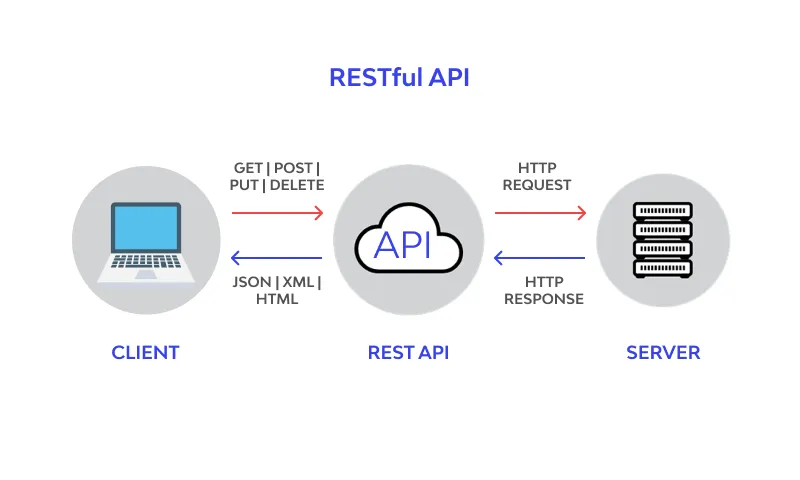
\includegraphics[width=0.9\linewidth]{Images/Chuong3/restful.png}%
            \end{center}

REST hoạt động chủ yếu dựa trên giao thức HTTP. Các thao tác cơ bản thường tương ứng với nhóm chức năng CRUD, bao gồm Create, Read, Update và Delete, tức là Tạo, Đọc, Cập nhật và Xóa dữ liệu.

Các phương thức HTTP thường dùng trong RESTful API gồm:
\begin{itemize}
    \item \textbf{GET (SELECT)}: Trả về một resource hoặc danh sách resource.
    \item \textbf{POST (CREATE)}: Tạo mới một resource.
    \item \textbf{PUT (UPDATE)}: Cập nhật thông tin cho resource.
    \item \textbf{DELETE (DELETE)}: Xóa một resource.
\end{itemize}

\textbf{Ưu điểm của RESTful API}:
\begin{itemize}
    \item Dễ hiểu, dễ học và có cách triển khai tương đối đơn giản.
    \item Cho phép tổ chức các ứng dụng phức tạp theo tài nguyên, giúp việc quản lý và sử dụng dữ liệu rõ ràng hơn.
    \item Hỗ trợ quản lý tải tốt nhờ tận dụng HTTP proxy server và cơ chế cache.
    \item Giúp các client mới như web, mobile hoặc ứng dụng bên thứ ba dễ dàng tích hợp với hệ thống.
    \item Cho phép sử dụng các phương thức HTTP tiêu chuẩn để truy xuất dữ liệu và gửi request.
    \item Hỗ trợ các định dạng dữ liệu linh hoạt như XML và JSON thông qua quá trình tuần tự hóa (serialize) dữ liệu.
    \item Có thể kết hợp với các giao thức xác thực như OAuth để bảo vệ request REST.
\end{itemize}

\subsection{Hệ quản trị cơ sở dữ liệu}
\subsubsection{PostgreSQL}
PostgreSQL là một hệ quản trị cơ sở dữ liệu quan hệ mã nguồn mở (Relational Database Management System – RDBMS) mạnh mẽ và phổ biến hiện nay. PostgreSQL tuân thủ chặt chẽ các chuẩn SQL và hỗ trợ đầy đủ các tính năng nâng cao như giao dịch (transaction), khóa (locking), chỉ mục (indexing) và ràng buộc toàn vẹn dữ liệu. Dữ liệu trong PostgreSQL được lưu trữ dưới dạng bảng (table) với các hàng và cột, phù hợp cho các hệ thống có cấu trúc dữ liệu chặt chẽ và mối quan hệ phức tạp.\\

Bên cạnh mô hình quan hệ truyền thống, PostgreSQL còn hỗ trợ kiểu dữ liệu JSON/JSONB, cho phép lưu trữ và truy vấn dữ liệu bán cấu trúc. Điều này giúp PostgreSQL trở thành một hệ quản trị cơ sở dữ liệu linh hoạt, có thể đáp ứng cả các yêu cầu của hệ thống dữ liệu quan hệ lẫn một phần nhu cầu của NoSQL. Nhờ khả năng mở rộng cao và độ ổn định tốt, PostgreSQL thường được sử dụng trong các hệ thống doanh nghiệp, ứng dụng web lớn và các hệ thống yêu cầu tính nhất quán dữ liệu cao.

\begin{center}
        
\includegraphics[width = 1.0\textwidth]{Images/Chuong3/postgresql.png}
\end{center}

\textbf{Ưu điểm của PostgreSQL:}
\begin{itemize}
    \item Tuân thủ chuẩn SQL cao: PostgreSQL hỗ trợ đầy đủ các chuẩn SQL hiện đại, giúp đảm bảo tính nhất quán và khả năng mở rộng của hệ thống.
    \item Hỗ trợ giao dịch mạnh mẽ: Cung cấp cơ chế ACID (Atomicity, Consistency, Isolation, Durability), đảm bảo an toàn và toàn vẹn dữ liệu.
    \item Xử lý tốt dữ liệu quan hệ phức tạp: Phù hợp với các hệ thống có nhiều bảng liên kết, ràng buộc khóa ngoại và logic nghiệp vụ phức tạp.
    \item Khả năng mở rộng và tùy biến cao: Hỗ trợ stored procedure, trigger, view và extension giúp mở rộng chức năng theo nhu cầu.
    \item Độ ổn định và tin cậy cao: PostgreSQL được đánh giá là một trong những hệ quản trị cơ sở dữ liệu ổn định nhất hiện nay, phù hợp cho các hệ thống quy mô lớn và dài hạn.
\end{itemize}


\textbf{Nhược điểm của PostgreSQL:}
\begin{itemize}
    \item Cấu hình và quản trị phức tạp hơn: So với các hệ quản trị NoSQL, PostgreSQL yêu cầu người quản trị có kiến thức chuyên sâu hơn để tối ưu hiệu năng.
    \item Khả năng mở rộng ngang hạn chế hơn NoSQL: Việc mở rộng theo chiều ngang (horizontal scaling) phức tạp hơn so với các hệ cơ sở dữ liệu NoSQL như MongoDB.
    \item Hiệu năng có thể giảm với dữ liệu cực lớn: Khi xử lý khối lượng dữ liệu rất lớn và truy vấn không được tối ưu, hiệu suất có thể bị ảnh hưởng.
\end{itemize}

\subsubsection{Supabase}
Supabase là một nền tảng Backend-as-a-Service (BaaS) mã nguồn mở, được xây dựng nhằm hỗ trợ các nhóm phát triển tạo ứng dụng web và mobile nhanh chóng hơn mà không cần tự xây dựng toàn bộ hạ tầng backend từ đầu. Supabase thường được xem là một giải pháp thay thế mã nguồn mở cho Firebase, nhưng điểm khác biệt quan trọng là Supabase sử dụng PostgreSQL làm cơ sở dữ liệu trung tâm. Nhờ đó, hệ thống vừa tận dụng được sức mạnh của cơ sở dữ liệu quan hệ, vừa cung cấp thêm nhiều dịch vụ backend hiện đại thông qua giao diện quản lý và API có sẵn.

Về bản chất, Supabase không chỉ là một hệ quản trị cơ sở dữ liệu đơn thuần mà là một nền tảng tích hợp nhiều thành phần phục vụ quá trình phát triển ứng dụng. Khi tạo một dự án Supabase, nhà phát triển có thể sử dụng PostgreSQL để lưu trữ dữ liệu, đồng thời tự động có các API để truy cập dữ liệu, cơ chế xác thực người dùng, lưu trữ tệp và các tính năng thời gian thực. Điều này giúp rút ngắn đáng kể thời gian triển khai backend, đặc biệt đối với các dự án cần phát triển nhanh hoặc có quy mô vừa và nhỏ.

\begin{center}
        
\includegraphics[width = 0.55\textwidth]{Images/Chuong3/supabase.png}
\end{center}

Các thành phần chính của Supabase bao gồm:
\begin{itemize}
    \item \textbf{Database}: Supabase sử dụng PostgreSQL làm cơ sở dữ liệu chính, cho phép lưu trữ dữ liệu dạng bảng, thiết lập quan hệ, khóa ngoại, chỉ mục và truy vấn bằng SQL.
    \item \textbf{Auto-generated API}: Supabase tự động tạo RESTful API và hỗ trợ truy cập dữ liệu thông qua client libraries, giúp frontend có thể tương tác với cơ sở dữ liệu một cách nhanh chóng.
    \item \textbf{Authentication}: Cung cấp hệ thống xác thực người dùng với email, mật khẩu, magic link và các nhà cung cấp đăng nhập bên thứ ba, hỗ trợ quản lý phiên đăng nhập và phân quyền.
    \item \textbf{Storage}: Cho phép lưu trữ và quản lý các tệp như hình ảnh, tài liệu hoặc tài nguyên người dùng tải lên, đồng thời có thể kết hợp với chính sách bảo mật để kiểm soát quyền truy cập.
    \item \textbf{Realtime}: Hỗ trợ lắng nghe thay đổi dữ liệu theo thời gian thực, phù hợp với các chức năng như thông báo, cập nhật trạng thái hoặc đồng bộ dữ liệu giữa nhiều client.
    \item \textbf{Edge Functions}: Cho phép triển khai các hàm backend nhẹ để xử lý logic phía máy chủ, tích hợp API bên ngoài hoặc thực hiện các tác vụ không nên xử lý trực tiếp ở frontend.
\end{itemize}

Một điểm mạnh quan trọng của Supabase là khả năng kết hợp giữa sự tiện lợi của nền tảng BaaS và tính chặt chẽ của PostgreSQL. Nhà phát triển vẫn có thể thiết kế schema, viết câu truy vấn SQL, tạo view, trigger hoặc function như khi làm việc với PostgreSQL truyền thống. Đồng thời, Supabase cung cấp giao diện quản trị trực quan giúp theo dõi bảng dữ liệu, chỉnh sửa bản ghi, cấu hình xác thực và quản lý storage dễ dàng hơn.

Trong các ứng dụng web hiện đại, Supabase thường được dùng như lớp backend phục vụ cho frontend được xây dựng bằng React, Vue, Angular hoặc các framework khác. Frontend có thể gọi trực tiếp đến API của Supabase để đọc, ghi và cập nhật dữ liệu. Để đảm bảo an toàn, Supabase hỗ trợ Row Level Security (RLS), cho phép định nghĩa chính sách truy cập dữ liệu ở cấp từng hàng trong bảng. Nhờ đó, hệ thống có thể kiểm soát người dùng nào được phép xem, thêm, sửa hoặc xóa dữ liệu.

\textbf{Ưu điểm của Supabase:}
\begin{itemize}
    \item Rút ngắn thời gian phát triển backend nhờ cung cấp sẵn cơ sở dữ liệu, API, xác thực, storage và realtime.
    \item Dựa trên PostgreSQL nên có khả năng lưu trữ dữ liệu quan hệ mạnh mẽ, hỗ trợ SQL và các ràng buộc toàn vẹn dữ liệu.
    \item Có giao diện quản trị trực quan, giúp việc tạo bảng, theo dõi dữ liệu và cấu hình dịch vụ trở nên thuận tiện.
    \item Hỗ trợ tích hợp tốt với các ứng dụng frontend hiện đại thông qua RESTful API và các thư viện client.
    \item Cung cấp cơ chế bảo mật Row Level Security, giúp kiểm soát quyền truy cập dữ liệu chi tiết hơn.
    \item Là nền tảng mã nguồn mở, có thể sử dụng dịch vụ đám mây của Supabase hoặc tự triển khai trên hạ tầng riêng khi cần.
\end{itemize}

\textbf{Nhược điểm của Supabase:}
\begin{itemize}
    \item Việc cấu hình bảo mật, đặc biệt là Row Level Security, đòi hỏi nhà phát triển hiểu rõ quyền truy cập dữ liệu để tránh rủi ro lộ thông tin.
    \item Với các hệ thống có logic nghiệp vụ phức tạp, vẫn cần xây dựng thêm backend riêng thay vì chỉ phụ thuộc vào API tự động.
    \item Khi ứng dụng tăng trưởng lớn, chi phí vận hành và yêu cầu tối ưu hiệu năng cơ sở dữ liệu cần được theo dõi cẩn thận.
\end{itemize}

\subsection{Cơ sở lý thuyết các bài toán đặc thù}

Bên cạnh các công nghệ nền tảng, hệ thống CoSpace ứng dụng một số lý thuyết khoa học máy tính và thuật toán chuyên sâu nhằm giải quyết triệt để các bài toán nghiệp vụ phức tạp.

\subsubsection{Độ tương đồng Jaccard (Jaccard Similarity) trong Partner Matching}

Trong không gian Co-working, việc kết nối các thành viên có năng lực hoặc nhu cầu hợp tác tương đồng đóng vai trò then chốt trong việc tạo dựng giá trị mạng lưới. Hệ thống sử dụng \textbf{Hệ số tương đồng Jaccard (Jaccard Similarity Coefficient)} để định lượng mức độ phù hợp giữa hai thành viên dựa trên tập hợp các thẻ kỹ năng (Skills) và sở thích chuyên môn (Interests).

Độ tương đồng Jaccard giữa hai tập hợp $A$ và $B$ được định nghĩa bằng tỷ số giữa kích thước phần giao và kích thước phần hợp của hai tập hợp:
\begin{equation}
    J(A, B) = \frac{|A \cap B|}{|A \cup B|} = \frac{|A \cap B|}{|A| + |B| - |A \cap B|}
\end{equation}

Hệ số $J(A, B)$ có giá trị nằm trong khoảng $[0, 1]$:
\begin{itemize}
    \item $J(A, B) = 0$ khi và chỉ khi hai tập hợp rời nhau hoàn toàn ($A \cap B = \emptyset$), tức hai thành viên không có điểm chung nào.
    \item $J(A, B) = 1$ khi và chỉ khi hai tập hợp trùng khớp hoàn toàn ($A = B$).
\end{itemize}

Trong hệ thống CoSpace, thuật toán được mở rộng bằng cách kết hợp có trọng số giữa điểm tương đồng kỹ năng ($J_{skills}$), điểm tương đồng sở thích ($J_{interests}$) và hệ số thưởng vị trí địa lý ($\alpha_{branch}$):
\begin{equation}
    \text{Score}(u_1, u_2) = w_1 \cdot J(\text{Skills}_{u_1}, \text{Skills}_{u_2}) + w_2 \cdot J(\text{Interests}_{u_1}, \text{Interests}_{u_2}) + \alpha_{branch}
\end{equation}
Trong đó $w_1 = 0.6$, $w_2 = 0.3$, và $\alpha_{branch} = 0.1$ nếu hai thành viên đang cùng ngồi làm việc tại một chi nhánh trong ngày. Điểm số tổng hợp được chuẩn hóa để xếp hạng top $N$ đối tác tiềm năng nhất cho người dùng.

\subsubsection{Mô hình ngôn ngữ lớn (LLM) và Google Gemini API}

Mô hình ngôn ngữ lớn (Large Language Model -- LLM) là các mạng nơ-ron học sâu dựa trên kiến trúc Transformer, được huấn luyện trước trên tập dữ liệu văn bản quy mô khổng lồ để hiểu ngữ cảnh, suy luận logic và sinh văn bản tự nhiên.

Hệ thống CoSpace tích hợp mô hình \textbf{Google Gemini 3.5 Flash} thông qua RESTful API để xây dựng Trợ lý ảo AI thông minh hỗ trợ khách hàng:
\begin{itemize}
    \item \textbf{Cơ chế System Instruction \& Prompt Engineering:} Hệ thống cung cấp cho mô hình ngữ cảnh chi tiết về bảng giá, các loại không gian, danh sách chi nhánh và chính sách hủy phòng của CoSpace. Nhờ đó, AI đóng vai trò như một nhân viên lễ tân am hiểu sâu sắc, phản hồi chính xác mọi thắc mắc của khách.
    \item \textbf{Xử lý ngôn ngữ tự nhiên đa ngữ:} Hỗ trợ nhận diện và phản hồi linh hoạt bằng Tiếng Việt và Tiếng Anh với ngữ điệu thân thiện, lịch thiệp.
    \item \textbf{Cơ chế tư vấn đặt phòng tự động:} AI có khả năng trích xuất các thông tin cần thiết từ đoạn chat của khách (loại phòng cần thuê, thời gian bắt đầu, số lượng người) để gợi ý vị trí chỗ ngồi phù hợp nhất kèm liên kết điều hướng đặt phòng trực tiếp.
\end{itemize}

\subsubsection{Chuẩn thanh toán VietQR Napas 24/7 và Webhook Idempotency}

Để thay thế hình thức chuyển khoản thủ công cần nhân viên đối soát, hệ thống tích hợp tiêu chuẩn \textbf{VietQR} thông qua cổng thanh toán trung gian \textbf{PayOS}:
\begin{itemize}
    \item \textbf{VietQR động (Dynamic VietQR):} Mã QR được tạo động cho từng giao dịch đặt phòng, chứa sẵn số tài khoản nhận tiền, số tiền chính xác và nội dung chuyển khoản mã hóa (chứa mã booking duy nhất). Khách hàng chỉ cần dùng ứng dụng ngân hàng quét mã là toàn bộ thông tin được điền tự động, loại bỏ hoàn toàn sai sót nhập số tiền hay nội dung.
    \item \textbf{Xử lý thông báo tức thời (Webhook Callback):} Khi tiền về tài khoản ngân hàng thông qua mạng lưới Napas 24/7, hệ thống PayOS gửi ngay một tín hiệu HTTP POST (Webhook) đến máy chủ CoSpace.
    \item \textbf{Nguyên tắc Idempotency (Tính duy nhất của giao dịch):} Trong môi trường mạng, Webhook có thể bị gửi lặp lại nhiều lần do cơ chế retry của bên thứ ba. Hệ thống áp dụng bảng kiểm soát giao dịch (\texttt{payments}) và cơ chế khóa bản ghi để đảm bảo mỗi giao dịch thành công chỉ được cập nhật trạng thái đơn hàng đúng một lần duy nhất, ngăn ngừa rủi ro cộng dồn thanh toán hoặc sai lệch kế toán.
    \item \textbf{Late Webhook Ghost Payment Recovery:} Trong trường hợp khách hàng thanh toán muộn sau khi đơn hàng đã hết hạn timeout 15 phút, hệ thống tự động ghi nhận tiền vào ví điểm hoàn tiền (Refund Wallet) cho khách hàng thay vì làm thất thoát tiền của người dùng.
\end{itemize}

\subsubsection{Cơ chế khóa hai tầng chống xung đột đặt phòng (Concurrency Control)}

Trong các nền tảng đặt phòng trực tuyến, xung đột đặt trùng chỗ (Overbooking) là vấn đề nghiêm trọng nhất. Hệ thống CoSpace xây dựng giải pháp phòng ngừa hai tầng:
\begin{enumerate}
    \item \textbf{Tầng 1 -- Khóa giao dịch cấp ứng dụng (PostgreSQL Advisory Xact Lock):} Khi một khách hàng bấm xác nhận đặt chỗ cho vị trí $W$ trong khoảng thời gian $[T_{start}, T_{end}]$, máy chủ Spring Boot thực thi hàm khóa logic \texttt{pg\_advisory\_xact\_lock(hashtext(concat(workspace\_id, date)))}. Khóa này tự động giữ đến khi transaction kết thúc, buộc mọi yêu cầu đặt phòng khác nhắm vào cùng vị trí đó phải xếp hàng chờ đợi, triệt tiêu hoàn toàn hiện tượng Race Condition ở tầng ứng dụng.
    \item \textbf{Tầng 2 -- Ràng buộc loại trừ cấp cơ sở dữ liệu (PostgreSQL Exclusion Constraint):} Ở cấp độ bảng \texttt{bookings}, hệ thống khai báo ràng buộc loại trừ sử dụng chỉ mục GiST trên kiểu dữ liệu \texttt{tstzrange}:
    \begin{equation*}
        \text{EXCLUDE USING gist (workspace\_id WITH =, tstzrange(start\_at, end\_at) WITH \&\&)}
    \end{equation*}
    Ràng buộc này đóng vai trò như một ``bức tường thép'' cuối cùng: ngay cả khi logic ứng dụng gặp sự cố, cơ sở dữ liệu PostgreSQL cũng sẽ tự động từ chối bất kỳ câu lệnh chèn nào có khoảng thời gian giao nhau (\&\&) trên cùng một mã không gian.
\end{enumerate}

\subsection{Cơ sở hạ tầng và DevOps (Cloud \& Containerization)}

\subsubsection{Container hóa với Docker}

Docker là nền tảng ảo hóa mức hệ điều hành (Containerization) cho phép đóng gói toàn bộ ứng dụng cùng môi trường thực thi, thư viện phụ thuộc và cấu hình hệ thống vào một khối duy nhất gọi là Docker Image. 

Hệ thống CoSpace ứng dụng kỹ thuật \textbf{Multi-stage build} để tối ưu hóa kích thước và bảo mật cho Backend Spring Boot:
\begin{itemize}
    \item \textbf{Giai đoạn 1 (Builder):} Sử dụng image \texttt{maven:3.9.9-eclipse-temurin-21} để tải thư viện và biên dịch mã nguồn Java thành file JAR.
    \item \textbf{Giai đoạn 2 (Runtime):} Chỉ sao chép file JAR thành phẩm sang image siêu nhẹ \texttt{eclipse-temurin:21-jre-alpine}. Image thành phẩm không chứa mã nguồn thô hay công cụ build, giúp giảm dung lượng image từ gần $800\text{MB}$ xuống dưới $250\text{MB}$, khởi động nhanh và hạn chế tối đa lỗ hổng bảo mật.
    \item \textbf{Tối ưu bộ nhớ JVM trong Container:} Cấu hình cờ \texttt{-XX:MaxRAMPercentage=75.0} giúp máy ảo Java tự động điều chỉnh kích thước bộ nhớ Heap linh hoạt theo dung lượng RAM được cấp phát bởi máy chủ Cloud, ngăn ngừa hiện tượng crash do tràn bộ nhớ (Out-Of-Memory).
\end{itemize}

\subsubsection{Hạ tầng Đám mây: Render Cloud và Vercel CDN Edge}

Nhằm đảm bảo tính sẵn sàng cao và chi phí vận hành tối ưu, hệ sinh thái CoSpace triển khai tách biệt hai phân hệ trên nền tảng đám mây:
\begin{itemize}
    \item \textbf{Backend API -- Render Cloud Platform:} Triển khai dưới dạng Web Service container hóa. Hệ thống hỗ trợ lắng nghe biến môi trường \texttt{\$\{PORT:8080\}} để gán cổng động do Render cấp phát, kích hoạt cơ chế Health Check tự động khởi động lại container khi có sự cố, và tích hợp Graceful Shutdown để chờ các tiến trình thanh toán dở dang hoàn tất trước khi dừng máy chủ.
    \item \textbf{Frontend SPA -- Vercel Edge CDN:} Triển khai dưới dạng Single Page Application (SPA). Mã nguồn giao diện được phân phối qua mạng lưới máy chủ biên (Edge Network) toàn cầu của Vercel, đảm bảo tốc độ tải trang cực nhanh và tự động gia hạn chứng chỉ bảo mật SSL/TLS.
\end{itemize}

\subsection{Bảng đối chiếu lý do lựa chọn công nghệ (Technology Justification Matrix)}

Để đảm bảo tính khoa học và minh bạch trong thiết kế hệ thống, nhóm tác giả xây dựng Bảng~\ref{tab:technology-justification} đối chiếu giữa công nghệ được lựa chọn và các giải pháp thay thế phổ biến trên thị trường.

\begin{table}[H]
\centering
\caption{Bảng đối chiếu lý do lựa chọn công nghệ (Technology Justification Matrix)}
\label{tab:technology-justification}
\renewcommand{\arraystretch}{1.3}
\begin{tabular}{|p{3cm}|p{3.5cm}|p{4.5cm}|p{4cm}|}
\hline
\textbf{Thành Phần} & \textbf{Công Nghệ Chọn} & \textbf{Giải Pháp Thay Thế} & \textbf{Lý Do Lựa Chọn Cốt Lõi} \\
\hline
\textbf{Backend Framework} & \textbf{Spring Boot 3 (Java 17/21)} & Node.js (Express), Python (Django), Go (Gin) & Tính chặt chẽ về hướng đối tượng và kiểu dữ liệu (Strongly-typed), hệ sinh thái bảo mật Spring Security mạnh mẽ, xử lý giao dịch tài chính ACID tin cậy. \\
\hline
\textbf{Frontend Framework} & \textbf{React 18 + Vite + TypeScript} & Next.js, Angular, Vue.js & Kiến trúc Component linh hoạt, Vite có tốc độ HMR và build nhanh gấp 10 lần Webpack, TypeScript đảm bảo an toàn kiểu dữ liệu ở Client, dễ dàng thao tác trực tiếp với DOM SVG. \\
\hline
\textbf{Cơ Sở Dữ Liệu} & \textbf{PostgreSQL 15 (Supabase)} & MySQL, MongoDB, Microsoft SQL Server & Hỗ trợ chỉ mục GiST và ràng buộc loại trừ thời gian (\texttt{tstzrange}) vượt trội, hỗ trợ lưu trữ JSONB linh hoạt, chuẩn ACID nghiêm ngặt. \\
\hline
\textbf{Cổng Thanh Toán} & \textbf{PayOS (VietQR) + MoMo} & VNPay, ZaloPay, Stripe & VietQR tương thích với $100\%$ ngân hàng tại Việt Nam, luồng tiền về trực tiếp tài khoản chủ chuỗi ngay lập tức không bị giam vốn, chi phí giao dịch thấp. \\
\hline
\textbf{Trí Tuệ Nhân Tạo} & \textbf{Google Gemini 3.5 Flash} & OpenAI GPT-4o, Anthropic Claude, Llama 3 & Chi phí truy xuất tối ưu, độ trễ phản hồi cực thấp (phù hợp cho chatbot thời gian thực), hỗ trợ hiểu ngữ cảnh Tiếng Việt xuất sắc. \\
\hline
\textbf{Hạ Tầng Triển Khai} & \textbf{Docker + Render + Vercel} & AWS (EC2/S3), Google Cloud, VPS truyền thống & Mô hình Cloud Native hiện đại, CI/CD tự động qua Git push, chi phí vận hành tối ưu cho giai đoạn khởi nghiệp, dễ dàng quản trị. \\
\hline
\end{tabular}
\end{table}
